\documentclass{imposter}
%\documentclass[landscape]{imposter}



%\usepackage{geometry}                		% See geometry.pdf to learn the layout options. There are lots.
%\geometry{landscape}                		% Activate for rotated page geometry
\usepackage[parfill]{parskip}    		% Activate to begin paragraphs with an empty line rather than an indent
%\usepackage{graphicx}				% Use pdf, png, jpg, or eps§ with pdflatex; use eps in DVI mode
								% TeX will automatically convert eps --> pdf in pdflatex		
															
\usepackage{wrapfig}								
\usepackage[font=scriptsize,labelfont=bf]{caption}
\usepackage[font=scriptsize]{subcaption}
\usepackage{float}
% \graphicspath{ {images/poster-eps/} }
\usepackage{amssymb}
\usepackage{amsmath}
\usepackage{bbm}

\usepackage{todonotes}

% \graphicspath{ {../papers/halfdisk/images/} }
\graphicspath{ {images/} }

\newcommand{\sotodo}{\todo[color=green]}
\newcommand{\sotodoinline}{\todo[color=green,inline=true]}
\newcommand{\bstodo}{\todo[color=pink]}
\newcommand{\bstodoinline}{\todo[color=pink,inline=true]}


\newcommand{\rightboxnoborder}[2]{{\rput[tr](82.1,#1){\psframebox[linecolor=white]{\begin{minipage}{38.9cm}#2\end{minipage}}}}}
\newcommand{\lefttboxnoborder}[2]{{\rput[tl](0,#1){\psframebox[linecolor=white]{\begin{minipage}{38.9cm}#2\end{minipage}}}}}
\newcommand{\rightboxreferences}[2]{{\rput[tr](82.1,#1){\psframebox[linecolor=titleframecolor]{\begin{minipage}{38.9cm}#2\end{minipage}}}}}
\newcommand{\leftboxreferences}[2]{{\rput[tl](0,#1){\psframebox[linecolor=titleframecolor]{\begin{minipage}{38.9cm}#2\end{minipage}}}}}


%SetFonts

%SetFonts

\usepackage{natbib}
\setlength{\bibsep}{0.0pt}
\usepackage{url}
\bibliographystyle{abbrv}

\newcommand{\bigO}{\mathcal{O}}
\newcommand{\half}{\frac{1}{2}}
\newcommand{\R}{\mathbb{R}}
\newcommand{\C}{\mathbb{C}}
\newcommand{\Z}{\mathbb{Z}}
\newcommand{\N}{\mathbb{N}}
\newcommand{\No}{\mathbb{N}_0}
\newcommand{\Ylm}{Y^m_l}
\newcommand{\Ylmfull}{Y^m_l(\theta,\varphi)}
\newcommand{\Plm}{\jac^m_l}
\newcommand{\costheta}{\cos\theta}
\newcommand{\sintheta}{\sin\theta}
\newcommand{\cosphi}{\cos\varphi}
\newcommand{\sinphi}{\sin\varphi}
\newcommand{\eimphi}{e^{im\varphi}}
\newcommand{\alphalm}{\alpha^m_l}
\newcommand{\clm}{c^m_l}
\newcommand{\ctilde}{\tilde{c}^m_l}
\newcommand{\ctildemod}{\tilde{c}^{|m|}_l}
\newcommand{\chat}{\hat{c}^m_l}
\newcommand{\chatmod}{\hat{c}^{|m|}_l}
\newcommand{\ddx}{\frac{\mathrm{d}}{\mathrm{d}x}}
\newcommand{\ddy}{\frac{\mathrm{d}}{\mathrm{d}y}}
\newcommand{\pddx}{\frac{\partial}{\partial x}}
\newcommand{\pddy}{\frac{\partial}{\partial y}}
\newcommand{\pddn}{\frac{\partial}{\partial n}}
\newcommand{\dmdxm}{\frac{\mathrm{d}^m}{\mathrm{d}x^m}}

\newcommand{\Atilde}{\tilde{A}_{l,m}}
\newcommand{\Btilde}{\tilde{B}_{l,m}}
\newcommand{\Dtilde}{\tilde{D}_{l,m}}
\newcommand{\Etilde}{\tilde{E}_{l,m}}
\newcommand{\Ftilde}{\tilde{F}_{l,m}}
\newcommand{\Gtilde}{\tilde{G}_{l,m}}
\newcommand{\Alm}{A_{l,m}}
\newcommand{\Blm}{B_{l,m}}
\newcommand{\Dlm}{D_{l,m}}
\newcommand{\Elm}{E_{l,m}}
\newcommand{\Flm}{F_{l,m}}
\newcommand{\Glm}{G_{l,m}}

\newcommand{\xione}{\xi^{(1)}_{n, \lambda}}
\newcommand{\xitwo}{\xi^{(2)}_{n, \lambda}}
\newcommand{\xithree}{\xi^{(3)}_{n, \lambda}}
\newcommand{\xifour}{\xi^{(4)}_{n, \lambda}}

\newcommand{\bigP}{\mathbb{P}}
\newcommand{\Pl}{\mathbb{P}_l}
\newcommand{\gradP}{T\mathbb{P}}
\newcommand{\gradPl}{T\mathbb{P}_l}
\newcommand{\gradY}{\nabla Y}
\newcommand{\gradYlm}{\nabla Y^m_l}
\newcommand{\gradpY}{\nabla^\perp Y}
\newcommand{\gradpYlm}{\nabla^\perp Y^m_l}

\newcommand{\Dlt}{D^\top_l}

\newcommand{\curlyy}{\bm{\mathcal{Y}}}
\newcommand{\blone}{\beta_{l, 1}}
\newcommand{\blzero}{\beta_{l, 0}}
\newcommand{\blmone}{\beta_{l, -1}}
\newcommand{\chivec}{\bm{\chi}_{1,m_s}}
\newcommand{\cgcoeff}{\mathcal{C}}

\newcommand{\alm}{a_{l,m}}
\newcommand{\blm}{b_{l,m}}
\newcommand{\dlm}{d_{l,m}}
\newcommand{\elm}{e_{l,m}}
\newcommand{\flm}{f_{l,m}}
\newcommand{\glm}{g_{l,m}}
\newcommand{\hlm}{h_{l,m}}
\newcommand{\jlm}{j_{l,m}}
\newcommand{\klm}{k_{l,m}}
\newcommand{\almperp}{a_{l,m}^\perp}
\newcommand{\blmperp}{b_{l,m}^\perp}
\newcommand{\dlmperp}{d_{l,m}^\perp}
\newcommand{\elmperp}{e_{l,m}^\perp}
\newcommand{\flmperp}{f_{l,m}^\perp}
\newcommand{\glmperp}{g_{l,m}^\perp}
\newcommand{\hlmperp}{h_{l,m}^\perp}
\newcommand{\jlmperp}{j_{l,m}^\perp}
\newcommand{\klmperp}{k_{l,m}^\perp}

\newcommand{\unitvec}{\hat{\bm{k}}}

\newcommand{\hdop}{H}
\newcommand{\bighdop}{\mathbb{\hdop}}
\newcommand{\hdopnk}{\hdop_{n,k}}
\newcommand{\hdopnkab}{\hdop_{n,k}^{(a,b)}}
\newcommand{\hdopab}{\hdop^{(a,b)}}
\newcommand{\Wab}{{W^{(a,b)}}}
\newcommand{\hdopmj}{\hdop_{m,j}}
\newcommand{\hdopmjab}{\hdop_{m,j}^{(a,b)}}
\newcommand{\alphaab}{\alpha^{(a,b)}}
\newcommand{\betaab}{\beta^{(a,b)}}
\newcommand{\bighdopab}{\bighdop^{(a,b)}}
\newcommand{\Dnt}{D^\top_n}
\newcommand{\Wii}{W^{(1,1)}}
\newcommand{\hdopii}{\hdop^{(1,1)}}
\newcommand{\bighdopii}{{\mathbb{\hdop}^{(1,1)}}}
\newcommand{\hdopoo}{\hdop^{(0,0)}}
\newcommand{\bighdopoo}{{\mathbb{\hdop}^{(0,0)}}}
\newcommand{\hdopoi}{\hdop^{(0,1)}}
\newcommand{\hdopio}{\hdop^{(1,0)}}
%\newcommand{\jac}{{\tilde P}}
\newcommand{\jac}{{P}}
\newcommand{\genjac}{R}
\newcommand{\genjacnmk}{\genjac_{n-k}}
\newcommand{\genjacmmj}{\genjac_{m-j}}
\newcommand{\genjacw}{w_\genjac}
\newcommand{\jacw}{w_P}
\newcommand{\normgenjac}{\omega_\genjac}
\newcommand{\normjac}{\omega_P}

\newcommand{\dx}{\frac{\partial}{\partial x}}
\newcommand{\dy}{\frac{\partial}{\partial y}}
\newcommand{\laplacewii}{\Delta_W^{(1,1)\to(1,1)}}
\newcommand{\laplacewtt}{\Delta_W^{(2,2)\to(0,0)}}
\newcommand{\laplaceoo}{\Delta^{(0,0)\to(2,2)}}
\newcommand{\biharmonic}{_2\Delta_W^{(2,2)\to(2,2)}}

\newcommand{\element}{\tau}
\newcommand{\refelement}{\hat{\tau}}
\newcommand{\FEset}{\mathcal{T}}
\newcommand{\bigW}{\mathbb{W}}
\newcommand{\bigWab}{\mathbb{W}^{(a,b)}}
\newcommand{\bigWii}{{\mathbb{W}^{(1,1)}}}
\newcommand{\bigQ}{\mathbb{Q}}
\newcommand{\bigQab}{\bigQ^{(a,b)}}
\newcommand{\Qab}{Q^{(a,b)}}


\newcommand{\hdopnkabc}{\hdop_{n,k}^{(a,b,c)}}
\newcommand{\hdopabc}{\hdop^{(a,b,c)}}
\newcommand{\Wabc}{{W^{(a,b,c)}}}
\newcommand{\hdopmjabc}{\hdop_{m,j}^{(a,b,c)}}
\newcommand{\alphaabc}{\alpha^{(a,b,c)}}
\newcommand{\betaabc}{\beta^{(a,b,c)}}
\newcommand{\bighdopabc}{\bighdop^{(a,b,c)}}
\newcommand{\Wiii}{W^{(1,1,1)}}
\newcommand{\hdopiii}{\hdop^{(1,1,1)}}
\newcommand{\bighdopiii}{{\mathbb{\hdop}^{(1,1,1)}}}
\newcommand{\hdopooo}{\hdop^{(0,0,0)}}
\newcommand{\bighdopooo}{{\mathbb{\hdop}^{(0,0,0)}}}
\newcommand{\hdopooi}{\hdop^{(0,0,1)}}
\newcommand{\hdopiio}{\hdop^{(1,1,0)}}
\newcommand{\laplacewiii}{\Delta_W^{(1,1,1)\to(1,1,1)}}
\newcommand{\laplacewttt}{\Delta_W^{(2,2,2)\to(0,0,0)}}
\newcommand{\laplaceooo}{\Delta^{(0,0,0)\to(2,2,2)}}
\newcommand{\biharmonictwo}{_2\Delta_W^{(2,2,2)\to(2,2,2)}}
\newcommand{\bigWiii}{{\mathbb{W}^{(1,1,1)}}}
\newcommand{\bigWabc}{\mathbb{W}^{(a,b,c)}}

\newcommand{\alphaabcd}{\alpha^{(a,b,c,d)}}
\newcommand{\betaabcd}{\beta^{(a,b,c,d)}}
\newcommand{\hdopnkabcd}{\hdop_{n,k}^{(a,b,c,d)}}
\newcommand{\hdopabcd}{\hdop^{(a,b,c,d)}}
\newcommand{\Wabcd}{{W^{(a,b,c,d)}}}
\newcommand{\hdopmjabcd}{\hdop_{m,j}^{(a,b,c,d)}}
\newcommand{\bighdopabcd}{\bighdop^{(a,b,c,d)}}
\newcommand{\bigWabcd}{\mathbb{W}^{(a,b,c,d)}}

\newcommand{\genjact}{\tilde{\genjac}}
\newcommand{\genjactnmk}{\genjact_{n-k}}
\newcommand{\genjactmmj}{\genjact_{m-j}}
\newcommand{\genjactw}{w_{\genjact}}
\newcommand{\normgenjact}{\omega_{\genjact}}

\newcommand{\xvec}{\mathbf{x}}

\usepackage{amsthm}

\newtheorem{proposition}{Proposition}
\newtheorem{lemma}{Lemma} 
\newtheorem{theorem}{Theorem} 
\newtheorem{definition}{Definition}
\newtheorem{condition}{Condition}
\newtheorem{algorithm}{Algorithm}
\newtheorem{corollary}{Corollary}

\def\condref#1{Condition~\ref{cond:#1}}


\def\addtab#1={#1\;&=}

\def\meeq#1{\def\ccr{\\\addtab}
%\tabskip=\@centering
 \begin{align*}
 \addtab#1
 \end{align*}
  }  
  
  \def\leqaddtab#1\leq{#1\;&\leq}
  \def\mleeq#1{\def\ccr{\\\addtab}
%\tabskip=\@centering
 \begin{align*}
 \leqaddtab#1
 \end{align*}
  }  


\def\vc#1{\mbox{\boldmath$#1$\unboldmath}}

\def\vcsmall#1{\mbox{\boldmath$\scriptstyle #1$\unboldmath}}

\def\vczero{{\mathbf 0}}


%\def\beginlist{\begin{itemize}}
%
%\def\endlist{\end{itemize}}


\def\pr(#1){\left({#1}\right)}
\def\br[#1]{\left[{#1}\right]}
\def\fbr[#1]{\!\left[{#1}\right]}
\def\set#1{\left\{{#1}\right\}}
\def\ip<#1>{\left\langle{#1}\right\rangle}
\def\iip<#1>{\left\langle\!\langle{#1}\right\rangle\!\rangle}

\def\norm#1{\left\| #1 \right\|}

\def\abs#1{\left|{#1}\right|}
\def\fpr(#1){\!\pr({#1})}

\def\Re{{\rm Re}\,}
\def\Im{{\rm Im}\,}

\def\floor#1{\left\lfloor#1\right\rfloor}
\def\ceil#1{\left\lceil#1\right\rceil}


\def\mapengine#1,#2.{\mapfunction{#1}\ifx\void#2\else\mapengine #2.\fi }

\def\map[#1]{\mapengine #1,\void.}

\def\mapenginesep_#1#2,#3.{\mapfunction{#2}\ifx\void#3\else#1\mapengine #3.\fi }

\def\mapsep_#1[#2]{\mapenginesep_{#1}#2,\void.}


\def\vcbr[#1]{\pr(#1)}


\def\bvect[#1,#2]{
{
\def\dots{\cdots}
\def\mapfunction##1{\ | \  ##1}
	\sopmatrix{
		 \,#1\map[#2]\,
	}
}
}

\def\vect[#1]{
{\def\dots{\ldots}
	\vcbr[{#1}]
}}

\def\vectt[#1]{
{\def\dots{\ldots}
	\vect[{#1}]^{\top}
}}

\def\Vectt[#1]{
{
\def\mapfunction##1{##1 \cr} 
\def\dots{\vdots}
	\begin{pmatrix}
		\map[#1]
	\end{pmatrix}
}}



\def\thetaB{\mbox{\boldmath$\theta$}}
\def\zetaB{\mbox{\boldmath$\zeta$}}


\def\newterm#1{{\it #1}\index{#1}}


\def\TT{{\mathbb T}}
\def\C{{\mathbb C}}
\def\R{{\mathbb R}}
\def\II{{\mathbb I}}
\def\F{{\mathcal F}}
\def\E{{\rm e}}
\def\I{{\rm i}}
\def\D{{\rm d}}
\def\dx{\D x}
\def\dy{\D y}
\def\CC{{\cal C}}
\def\DD{{\cal D}}
\def\U{{\mathbb U}}
\def\A{{\cal A}}
\def\K{{\cal K}}
\def\DTU{{\cal D}_{{\rm T} \rightarrow {\rm U}}}
\def\LL{{\cal L}}
\def\B{{\cal B}}
\def\T{{\cal T}}
\def\W{{\cal W}}


\def\tF_#1{{\tt F}_{#1}}
\def\Fm{\tF_m}
\def\Fab{\tF_{\alpha,\beta}}
\def\FC{\T}
\def\FCpmz{\FC^{\pm {\rm z}}}
\def\FCz{\FC^{\rm z}}

\def\tFC_#1{{\tt T}_{#1}}
\def\FCn{\tFC_n}

\def\rmz{{\rm z}}

\def\chapref#1{Chapter~\ref{Chapter:#1}}
\def\secref#1{Section~\ref{Section:#1}}
\def\exref#1{Exercise~\ref{Exercise:#1}}
\def\lmref#1{Lemma~\ref{Lemma:#1}}
\def\propref#1{Proposition~\ref{Proposition:#1}}
\def\warnref#1{Warning~\ref{Warning:#1}}
\def\thref#1{Theorem~\ref{Theorem:#1}}
\def\defref#1{Definition~\ref{Definition:#1}}
\def\probref#1{Problem~\ref{Problem:#1}}
\def\corref#1{Corollary~\ref{Corollary:#1}}
\def\appref#1{Appendix~\ref{Appendix:#1}}

\def\sgn{{\rm sgn}\,}
\def\Ai{{\rm Ai}\,}
\def\Bi{{\rm Bi}\,}
\def\wind{{\rm wind}\,}
\def\erf{{\rm erf}\,}
\def\erfc{{\rm erfc}\,}
\def\qqquad{\qquad\quad}
\def\qqqquad{\qquad\qquad}


\def\spand{\hbox{ and }}
\def\spodd{\hbox{ odd}}
\def\speven{\hbox{ even}}
\def\qand{\quad\hbox{and}\quad}
\def\qqand{\qquad\hbox{and}\qquad}
\def\qfor{\quad\hbox{for}\quad}
\def\qqfor{\qquad\hbox{for}\qquad}
\def\qas{\quad\hbox{as}\quad}
\def\qqas{\qquad\hbox{as}\qquad}
\def\qor{\quad\hbox{or}\quad}
\def\qqor{\qquad\hbox{or}\qquad}
\def\qqwhere{\qquad\hbox{where}\qquad}



%%% Words

\def\naive{na\"\i ve\xspace}
\def\Jmap{Joukowsky map\xspace}
\def\Mobius{M\"obius\xspace}
\def\Holder{H\"older\xspace}
\def\Mathematica{{\sc Mathematica}\xspace}
\def\apriori{apriori\xspace}
\def\WHf{Weiner--Hopf factorization\xspace}
\def\WHfs{Weiner--Hopf factorizations\xspace}

\def\Jup{J_\uparrow^{-1}}
\def\Jdown{J_\downarrow^{-1}}
\def\Jin{J_+^{-1}}
\def\Jout{J_-^{-1}}



\def\bD{\D\!\!\!^-}




\def\questionequals{= \!\!\!\!\!\!{\scriptstyle ? \atop }\,\,\,}

\def\elll#1{\ell^{\lambda,#1}}
\def\elllp{\ell^{\lambda,p}}
\def\elllRp{\ell^{(\lambda,R),p}}


\def\elllRpz_#1{\ell_{#1{\rm z}}^{(\lambda,R),p}}


\def\sopmatrix#1{\begin{pmatrix}#1\end{pmatrix}}

\def\socases#1{\begin{cases} #1 \end{cases}}


\def\Problem#1#2\par{\begin{problem}\label{pb:#1} #2\end{problem}}
\def\Theorem#1#2\par{\begin{theorem}\label{th:#1} #2\end{theorem}}
\def\Conjecture#1#2\par{\begin{conjecture}\label{conj:#1} #2\end{conjecture}}
\def\Proposition#1#2\par{\begin{proposition}\label{prop:#1} #2\end{proposition}}
\def\Definition#1#2\par{\begin{definition}\label{def:#1} #2\end{definition}}
\def\Corollary#1#2\par{\begin{corollary}\label{cr:#1} #2\end{corollary}}
\def\Lemma#1#2\par{\begin{lemma}\label{lm:#1} #2\end{lemma}}
\def\Example#1#2\par{\begin{example}\label{ex:#1} #2\end{example}}
\def\Remark #1\par{\begin{remark*}#1\end{remark*}}


\def\Proof{\begin{proof}}
\def\mqed{\end{proof}}


\def\Figuretwow[#1,#2]#3#4\par{
\begin{figure}[tb]
\begin{center}{
\includegraphics[width=#3]{Figures/#1}\includegraphics[width=#3]{Figures/#2}}
\end{center}
\caption{#4}\label{fig:#1} 
\end{figure}
}


\usepackage{listings}

\title{Sparse Spectral Methods for PDEs on Disk-Slices, Trapeziums and Spherical Bands}
\author{Ben Snowball, Sheehan Olver}
\department{Department of Mathematics, Imperial College London with the MPE CDT}

%% Primary university logo.
%\logo{imperial.eps}
% Secondary logos (not supported in all poster styles)
%\logoa{AMCG.eps}

%% Options to set colors of multiple poster features.
\titlecolor{named}{Blue}
\postercolor{named}{Blue}
%\pagecolor{green}

\posterstyle{mpecdtstyle}


% This sets up boxes to have nice rounded corners and somewhat thicker lines
% than the default.
\psset{linecolor=postercolor,linewidth=.2,cornersize=absolute,linearc=0.5,framesep=0.5}



\begin{document}
%\showgrid

% LHS

  \leftbox{96}{
        \section{Introduction}
        
In recent years, \textbf{sparse spectral methods} (SSMs) have been derived using hierarchies of classical \textbf{orthogonal polynomials} (OPs) on intervals, disks, and triangles (e.g. \cite{olver2019triangle}). We extend this methodology to a hierarchy of non-classical orthogonal polynomials on \textbf{disk slices} (e.g. a half-disk) and \textbf{trapeziums}. Sparsity is guaranteed due to the boundary being defined by an algebraic curve, and the entries of partial differential operators can be determined using formulae in terms of (non/semi-classical) univariate OPs. This work will lead to investigating \textbf{p-FEM} using disk-slice or trapezium shaped elements, and further to solving PDEs on the 3D \textbf{spherical band} or \textbf{polar cap}.
    }
    
    
  \leftbox{77.5}{
      \section{Construction of OPs on the disk-slice and trapezium}

Here, we develop SSMs for solving linear PDEs on a special class of geometries that includes disk-slices and trapeziums:
\begin{align*}
	\Omega := \{(x,y) \in \R^2 \quad | \quad \alpha < x < \beta, \: \gamma \rho(x) < y < \delta \rho(x)\}
\end{align*}
where either of the following conditions hold:
\begin{condition}\label{cond:trap}
	$\rho$ is a degree 1 polynomial.
\end{condition}
\begin{condition}\label{cond:disk}
	$\rho$ is the square root of a non-negative degree $\le$ 2 polynomial, and $-\gamma = \delta > 0$.
\end{condition}

We can construct 2D orthogonal polynomials on $\Omega$ by specialising the Proposition in \cite[p55--56]{dunkl2014orthogonal} in the following.

\begin{definition}
Let $\{\genjac_n^{(a,b,c)}\}$ be a three-parameter family of 1D OPs orthonormal w.r.t. the weight $\genjacw^{(a,b,c)}(x) := (\beta - x)^a \: (x - \alpha)^{b} \: \rho(x)^{c}$ on $(\alpha,\beta)$, and let $\{\jac_n^{(a,b,c)}\}$ be a two-parameter family of 1D OPs orthonormal w.r.t. the weight $\jacw^{(a,b)}(x) := (\delta-x)^a \: (x - \gamma)^b$ on $(\gamma,\delta)$.

Define the \textbf{four-parameter 2D orthogonal polynomial family on $\Omega$} via:
\begin{align*}
	\hdopnk^{(a,b,c,d)}(x,y) := \genjacnmk^{(a, b, c+d+2k+1)}(x) \: \rho(x)^k \: \jac_k^{(d,c)}\fpr(\frac{y}{\rho(x)}), \quad (x,y) \in \Omega, 
\end{align*}
which are orthogonal w.r.t. the weight
\begin{align*}
	W^{(a,b,c,d)}(x,y) := \genjacw^{(a,b,c+d)}(x) \: \jacw^{(d,c)}\fpr(\frac{y}{\rho(x)}), \quad (x,y) \in \Omega,
\end{align*}
\end{definition}

A function $f: \Omega \to \R$ can then be expressed as a vector $\textbf{f} = \{f_{n,k}\}$ of coefficients in our OP basis: $f(x,y) \approx \sum_{n=0}^N \sum_{k=0}^n f_{n,k} \; \hdopnkabcd(x,y)$, for sufficiently large $N$ (with equality if $f$ is a degree $N$ polynomial).

\subsection{Example: Disk-Slice}
	
For a disk-slice, we have $(\gamma,\delta) := (-1,1)$ and $\rho(x) := (1-x^2)^{\half}$. Thus we can simply remove the need for including a fourth parameter $d$, since we are in Condition \ref{cond:disk}:
\begin{align*}\label{eq:diskpolys}
	\hdopnkabc(x,y) := \genjacnmk^{(a, b, 2c+2k+1)}(x) \: \rho(x)^k \: \jac_k^{(c,c)}\fpr(\frac{y}{\rho(x)}), \quad (x,y) \in \Omega
\end{align*}

\noindent{\bf Remark}: In this case the weight $\jacw(x)$ is an ultraspherical weight, and the corresponding OPs are the normalized Jacobi polynomials $\{\jac_n^{(b, b)}\}$, while $\genjacw(x)$ is non-classical (it is in fact semi-classical, see \cite[\S5]{magnus1995painleve}).

    }	
    

    \rightbox{96}{
    	\section{Sparse Operators}		

\begin{wrapfigure}{L}{0.4\textwidth}
\center
\begin{tikzpicture} 
% Box/square (4x4)
\draw[black,solid,ultra thin] (0,0)--(0,4);
\draw[black,solid,ultra thin] (0,0)--(4,0);
\draw[black,solid,ultra thin] (4,0)--(4,4);
\draw[black,solid,ultra thin] (0,4)--(4,4);
% Dots
\draw[black,fill=black] (0,0) circle (.5ex);
\draw[black,fill=black] (2,2) circle (.5ex);
\draw[black,fill=black] (4,4) circle (.5ex);
\draw[black,fill=black] (0,2) circle (.5ex);
\draw[black,fill=black] (0,4) circle (.5ex);
% Arrows
\draw[black,thick,->] (0.2,0.2)--(1.8,1.8);
\draw[black,thick,->] (2.2,2.2)--(3.8,3.8);
\draw[black,thick,->] (0,0.2)--(0,1.8);
\draw[black,thick,->] (0,2.2)--(0,3.8);
\draw [black,thick,->] (0.2,4.2) to [out=20,in=160] (3.8,4.2);
% Node (parameter) labels
\draw[] (0,-0.5) node[anchor=east] {$(0,0,0)$};
\draw[] (0,4.5) node[anchor=east] {$(0,0,2)$};
\draw[] (4,-0.5) node[anchor=west] {$(2,2,0)$};
\draw[] (4,4.5) node[anchor=west] {$(2,2,2)$};
% Arrow labels
\draw[] (1.5,1.5) node[anchor=north] {$\tfrac{\partial}{\partial x}$};
\draw[] (3.5,3.5) node[anchor=north] {$\tfrac{\partial}{\partial x}$};
\draw[] (-2,1) node[anchor=west] {$\tfrac{\partial}{\partial y}$};
\draw[] (-2,3) node[anchor=west] {$\tfrac{\partial}{\partial y}$};
% The key and headings
\draw[] (2,5.3) node[anchor=south] {Parameter Conversion};
\end{tikzpicture} 
\label{fig:Laplace} 
\end{wrapfigure}

The construction leads to \textbf{sparse Jacobi operator matrices} for multiplication by $x$, $y$. We can hence derive a recurrence relation and construct methods to expand functions in our OP basis, evaluate functions using the \textbf{Clenshaw algorithm}, derive sparse relations for partial derivatives of the OPs. This is implemented in a code library that utilises ApproxFun \cite{ApproxFun}. \\
	
We are also guaranteed sparsity of the partial differential relationships, and hence obtain \textbf{sparse differential operator matrices} with \textbf{banded-block-banded} structure. \\

\begin{wrapfigure}{R}{0.7\textwidth}
	\centering
	\begin{subfigure}{0.2\textwidth}
	\centering
	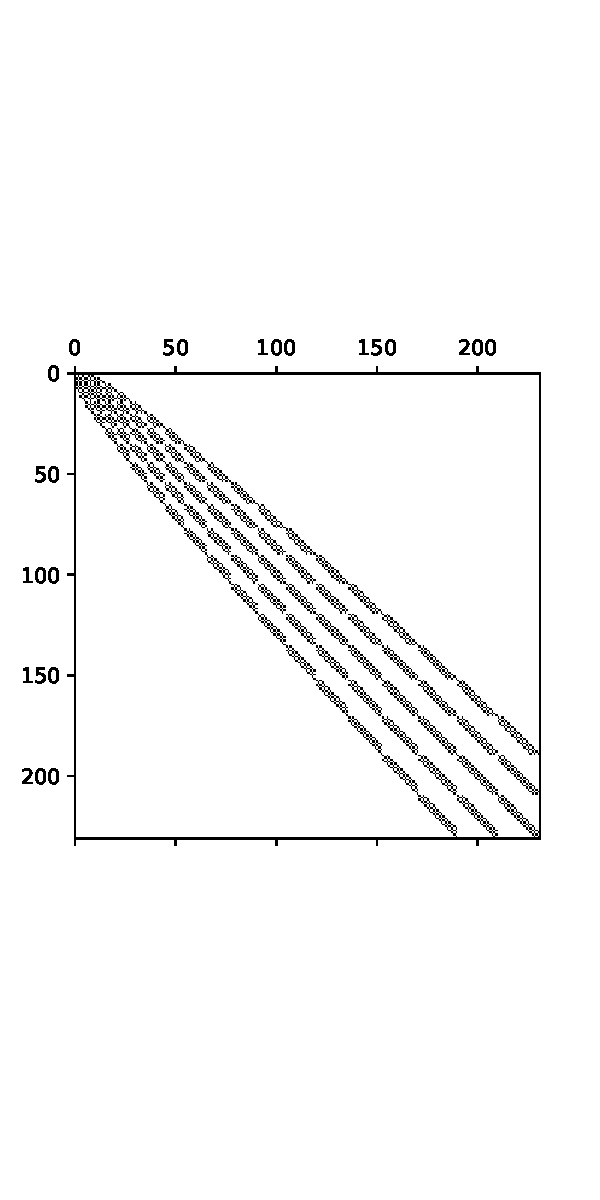
\includegraphics[scale=0.6]{sparsityoflaplacian-w11-diskslice-alpha=0p2-beta=0p8}
        \centering
	\end{subfigure}
	\begin{subfigure}{0.2\textwidth}
	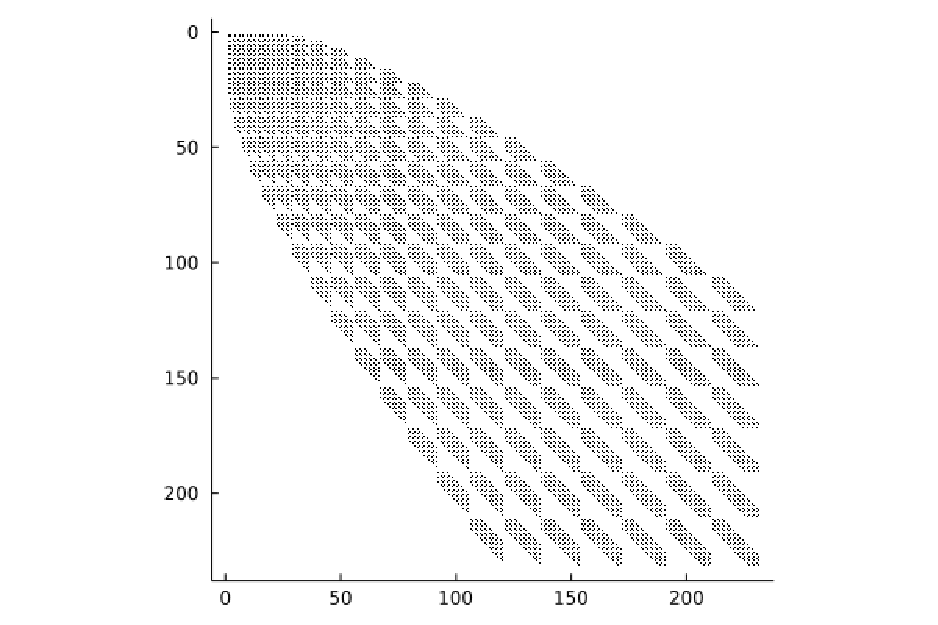
\includegraphics[scale=0.6]{sparsityofhelmholtz-diskslice-alpha=0p2-beta=0p8}
        \centering
	\end{subfigure}
	\begin{subfigure}{0.2\textwidth}
	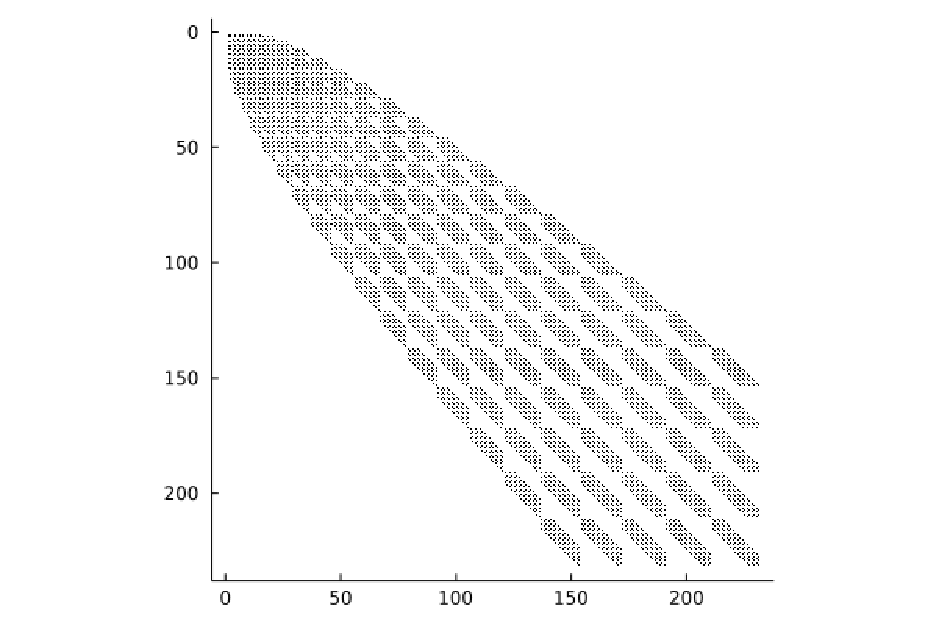
\includegraphics[scale=0.6]{sparsityofbiharmonic-diskslice-alpha=0p2-beta=0p8}
        \centering
	\end{subfigure}
	\captionsetup{width=.8\linewidth}
    	\caption{"Spy" plots of (differential) operator matrices, showing their sparsity. Left: the Laplace operator. Centre: the weighted variable coefficient Helmholtz operator $\Delta + k^2 \: v$ for $v(x,y) = 1 - (3(x-1)^2 + 5y^2)$ and $k = 200$. Right: the biharmonic operator.}
        \label{fig:sparsity}
        \centering
\end{wrapfigure}

The \textbf{Laplacian operator} for example can be constructed as a combination of the sparse partial differential operators and \textbf{sparse parameter increment/decrement operators}. The incrementing and decrementing of parameters here is analogous to other well known OP families' derivatives (see \cite[(18.9.3)]{DLMF}, \cite{olver2018recurrence}).

}


	\rightboxnoborder{51}{	

%$ $
%
%\begin{wrapfigure}{L}{\textwidth}
%	\centering
%        \begin{subfigure}{0.35\linewidth}
%        \centering
%        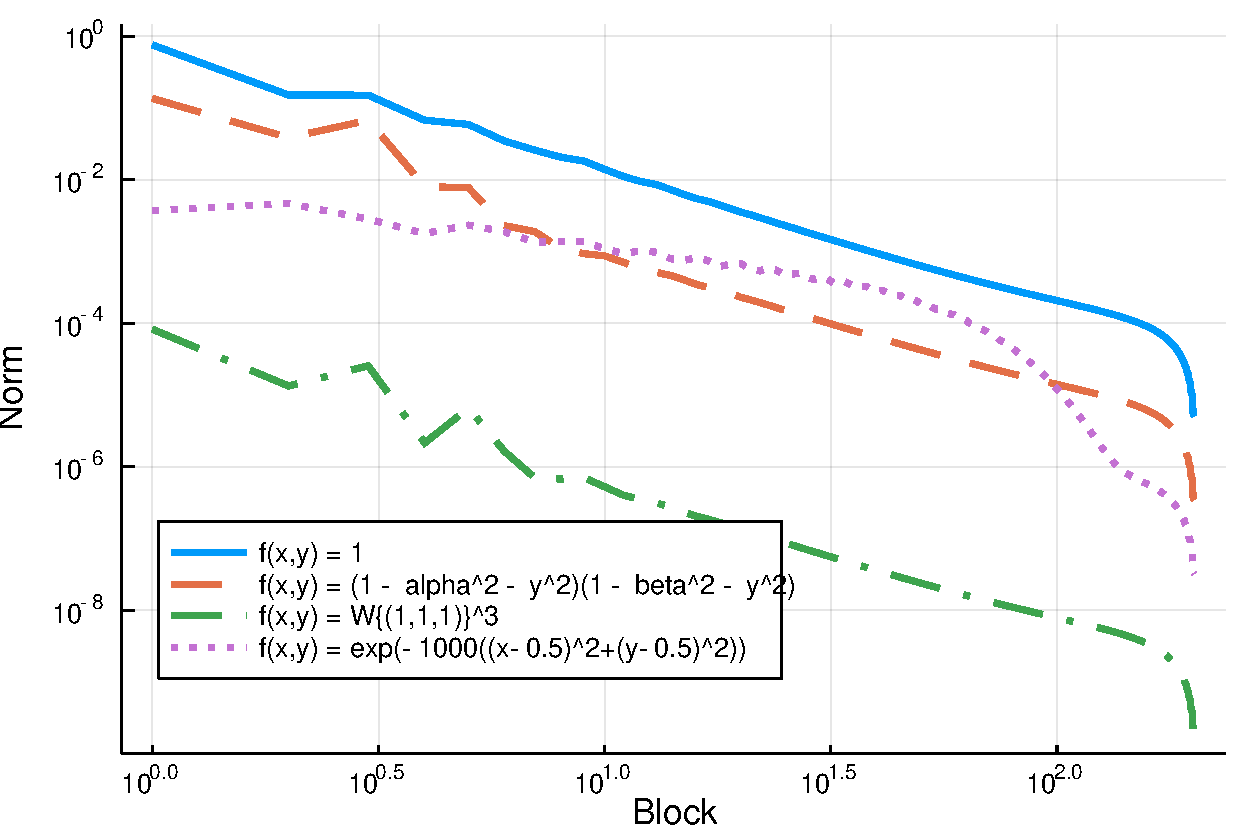
\includegraphics[scale=0.6]{solutionblocknorms-poisson-diskslice-alpha=0p2-beta=0p8-N=200}
%        \end{subfigure}
%        \centering
%        \begin{subfigure}{.15\linewidth}
%        \centering
%        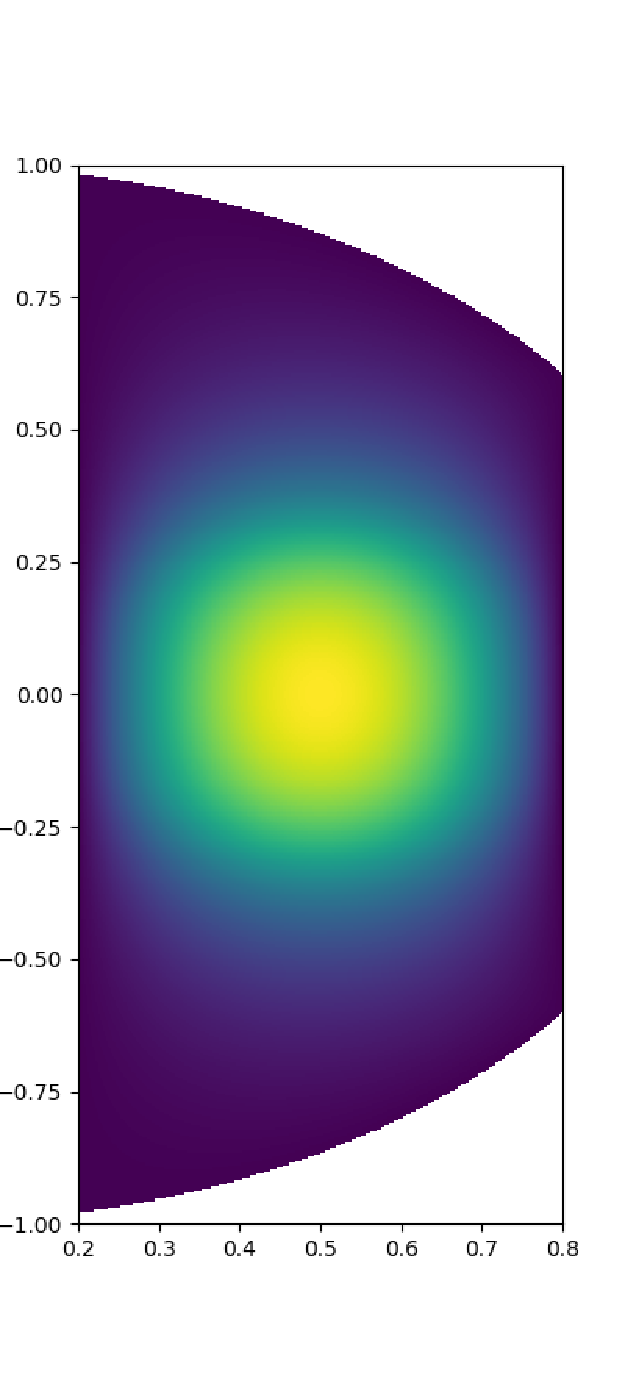
\includegraphics[scale=0.55]{solution-poisson-diskslice-alpha=0p2-beta=0p8}
%        \end{subfigure}
%        \centering
%        \begin{subfigure}{.15\linewidth}
%        \centering
%        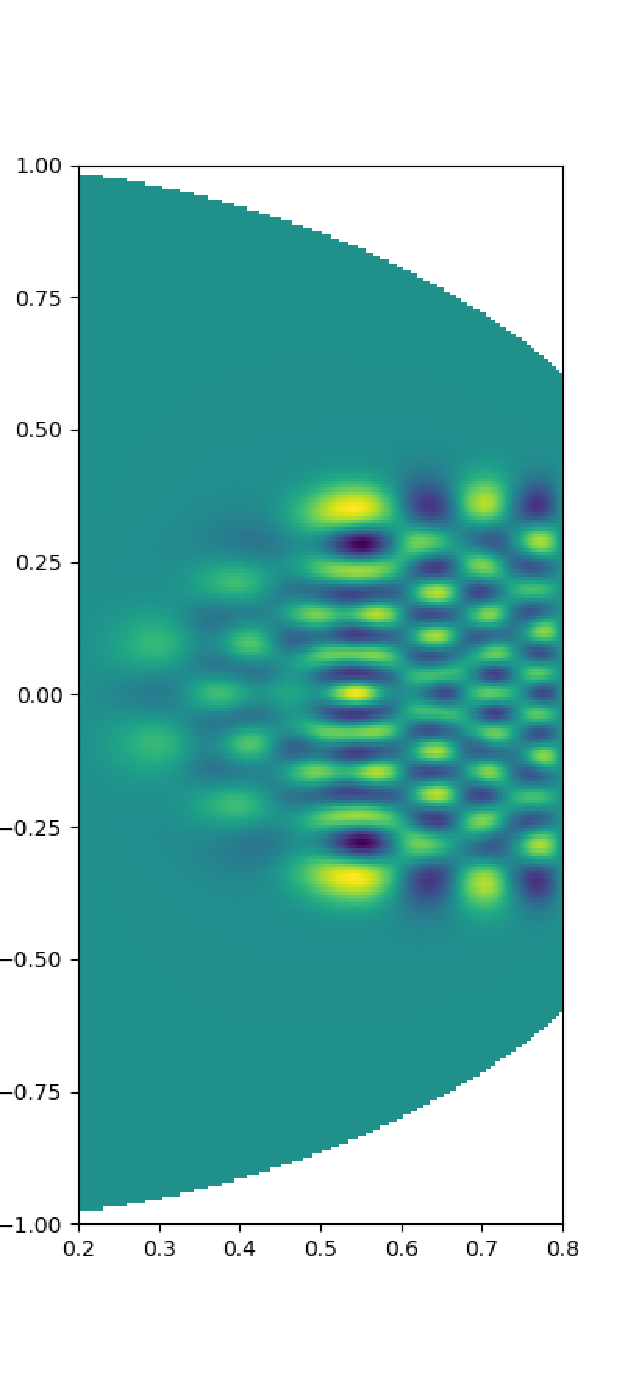
\includegraphics[scale=0.55]{solution-helmholtz-diskslice-alpha=0p2-beta=0p8-k=100-n=300}
%        \end{subfigure}
%        \centering
%        \begin{subfigure}{.15\linewidth}
%        \centering
%        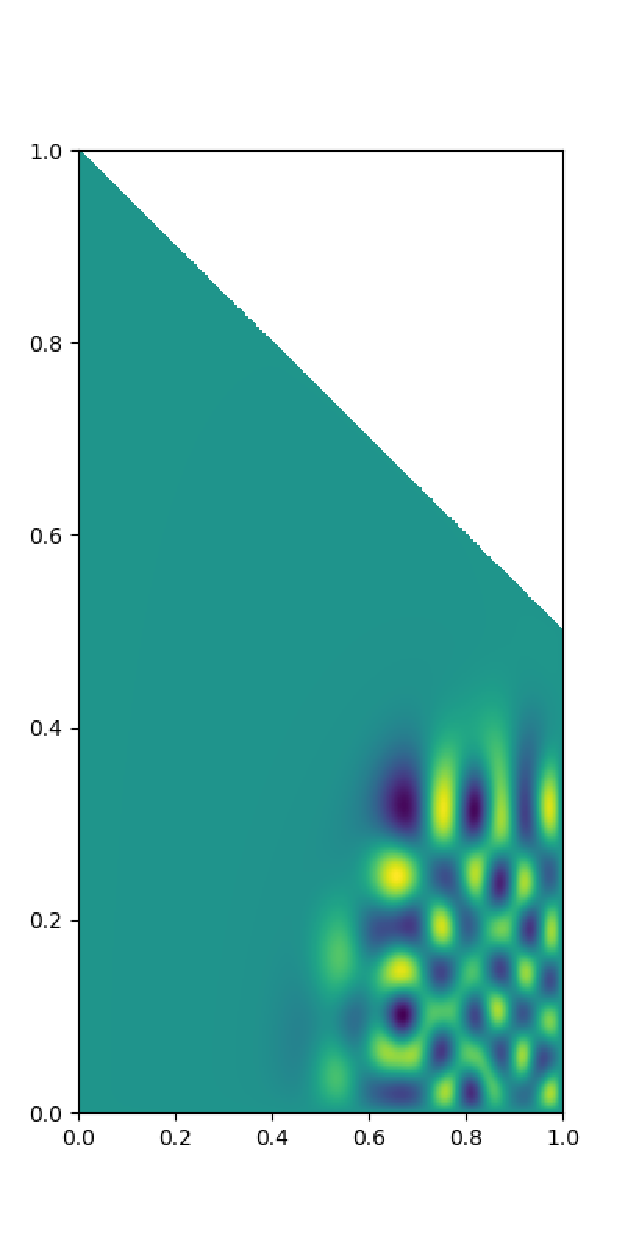
\includegraphics[scale=0.58]{solution-trapezium-helmholtz-k=100-n=1500}
%        \end{subfigure}
%        \centering
%        \captionsetup{width=.8\linewidth}
%        \caption{Right: The norms of each block of the computed solution of the Poisson equation with the given right hand side functions. This demonstrates algebraic convergence with the rate dictated by the decay at the corners, with spectral convergence observed when the right-hand side vanishes to all orders. Right 3: The computed solutions $u$ with zero BCs to: Left: $\Delta u = f$, $f(x,y) = 1 + \text{erf}(5(1 - 10((x - 0.5)^2 + y^2)))$. Centre: $\Delta u + k^2 \: v \: u = f$, $f(x,y) = x(1-x^2-y^2)e^x$, $v(x,y) = 1 - (3(x-1)^2 + 5y^2)$, $k = 100$. Right: $\Delta u + k^2 \: v \: u = f$, $f(x,y) = (1-x) \: x \: y \: (1- \half x - y) \: e^x$, $v(x,y) = 1 - (3(x-1)^2 + 5y^2)$, $k = 100$.}
%        \centering
%\end{wrapfigure}
%
%$$
%$$

\begin{center}
	\includegraphics[scale=0.73]{solutionblocknorms-poisson-diskslice-alpha=0p2-beta=0p8-N=950-f64}
	\quad
	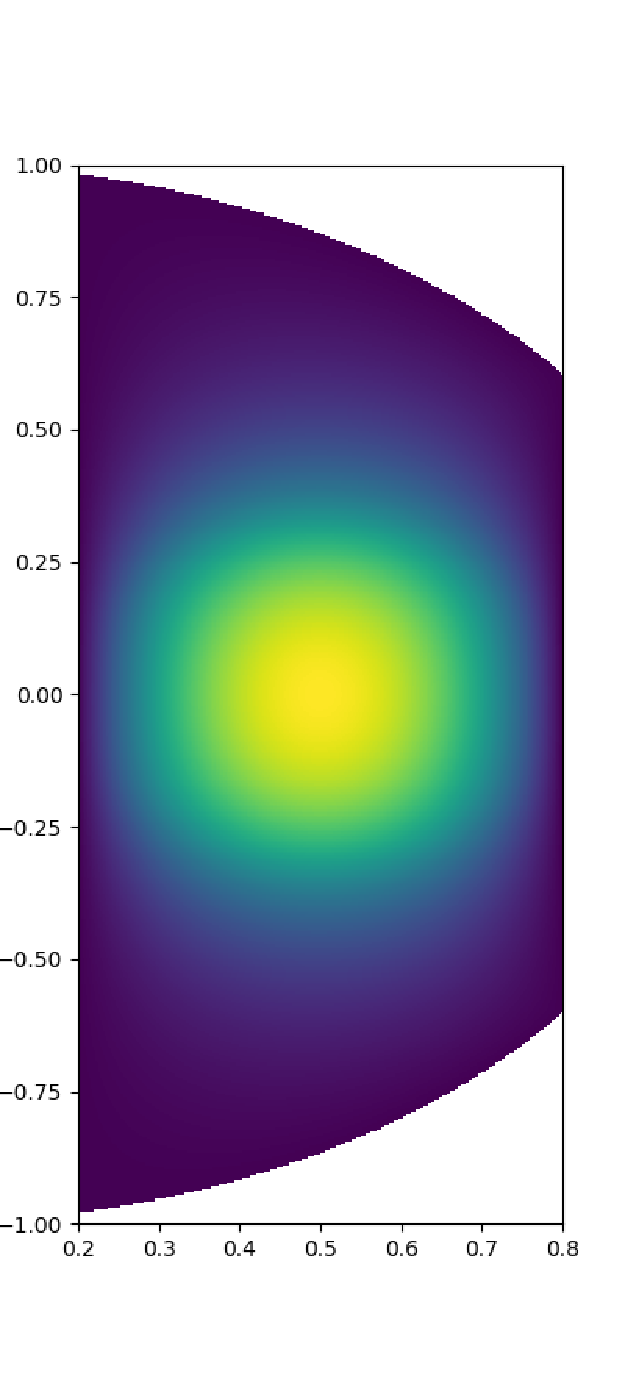
\includegraphics[scale=0.65]{solution-poisson-diskslice-alpha=0p2-beta=0p8}
	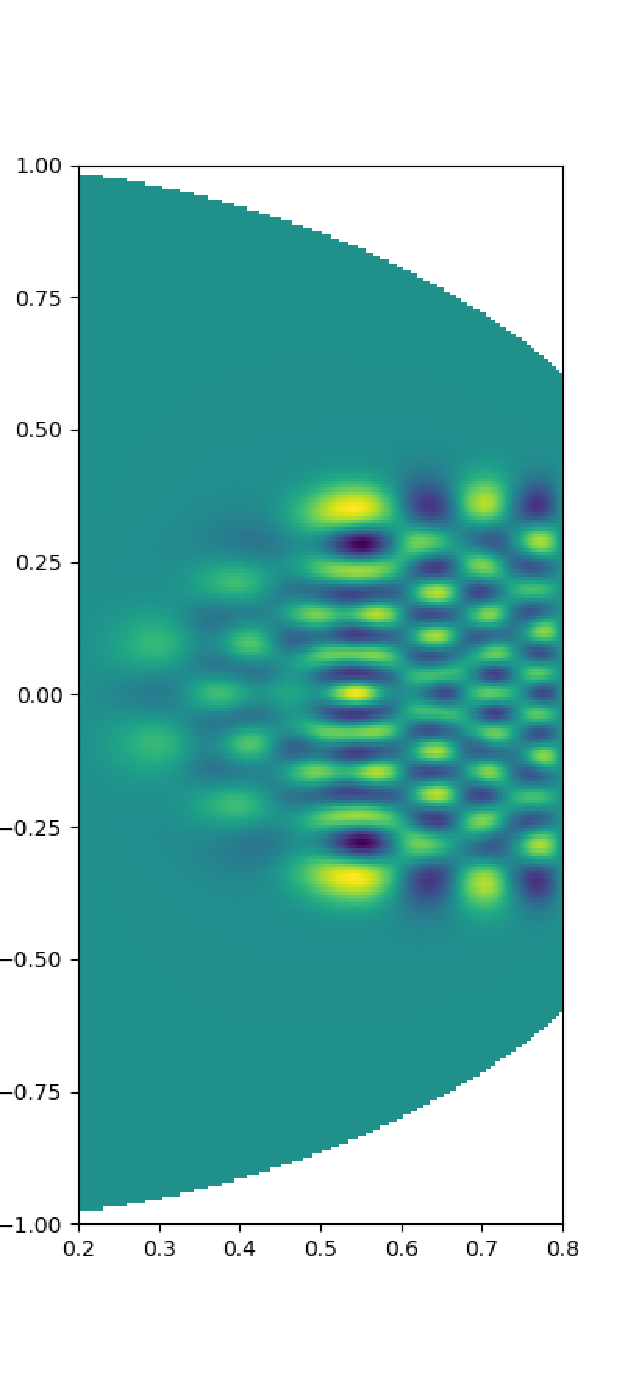
\includegraphics[scale=0.65]{solution-helmholtz-diskslice-alpha=0p2-beta=0p8-k=100-n=300}
	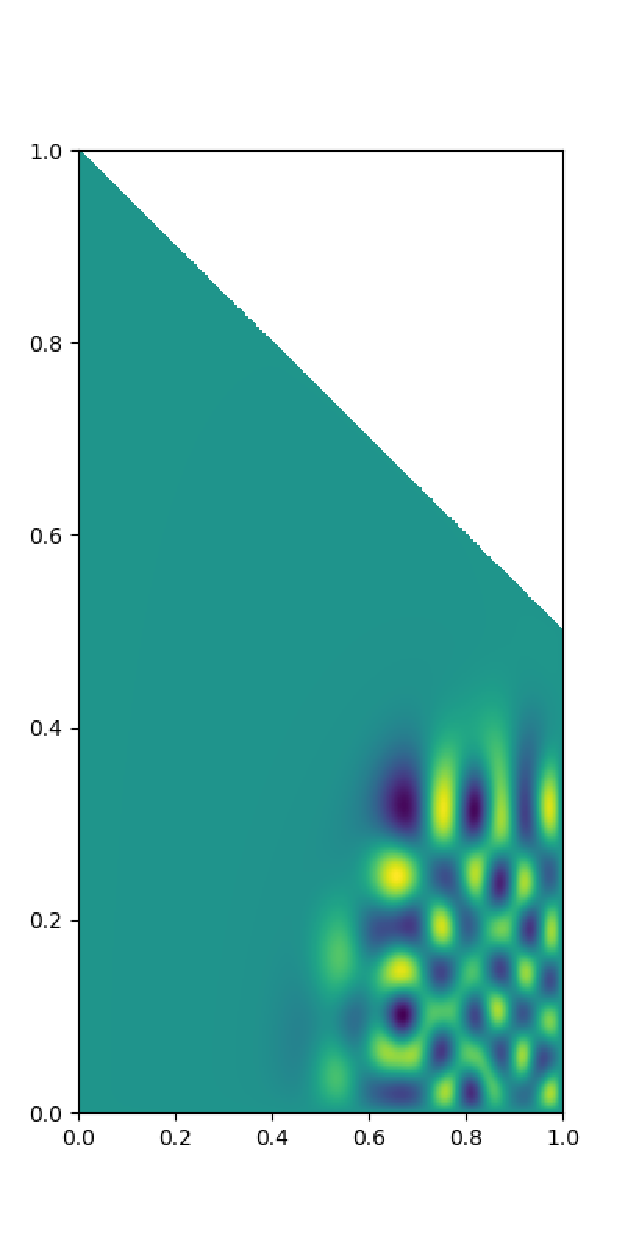
\includegraphics[scale=0.69]{solution-trapezium-helmholtz-k=100-n=1500}
\end{center}
$ $\\
\scriptsize{\textbf{Figure 2: } Right: The norms of each block of the computed solution of the Poisson equation with the given right hand side functions. This demonstrates \textbf{algebraic convergence} with the rate dictated by the decay at the corners, with spectral convergence observed when the right-hand side vanishes to all orders. Right 3: The computed solutions $u$ with zero BCs to: Left: $\Delta u = f$, $f(x,y) = 1 + \text{erf}(5(1 - 10((x - 0.5)^2 + y^2)))$. Centre: $\Delta u + k^2 \: v \: u = f$, $f(x,y) = x(1-x^2-y^2)e^x$, $v(x,y) = 1 - (3(x-1)^2 + 5y^2)$, $k = 100$. Right: $\Delta u + k^2 \: v \: u = f$, $f(x,y) = (1-x) \: x \: y \: (1- \half x - y) \: e^x$, $v(x,y) = 1 - (3(x-1)^2 + 5y^2)$, $k = 100$.}

}

    
      \rightbox{28}{
      \section{OPs on the spherical cap and spherical band}
      
We can develop a similar framework on the spherical cap and spherical band. The 3D OPs will be simply the two-parameter family given by
\begin{align*}
	\tilde{Q}^{(a,b)}_{n,k}(x, y, z) \equiv \Qab_{n,k}(\theta, z) &:= \genjac_{n-k}^{(a,b,2k+1)}(z) \: \rho(z)^k \: e^{i k \theta}, \quad (x,y,z) \in \Omega
\end{align*}
where $\Omega := \{(x,y,z) \in \R^3 \quad | \quad z \in (\alpha, \beta), \: ||(x,y)|| = \rho(z)\}$, and $\theta, \phi$ are defined according to $x = \cos \theta \sin \phi$, $y = \sin \theta \sin \phi$, $z = \cos \phi$. Note the comparison to the \textbf{spherical harmonics} defined on the whole sphere.

    }
    
    
    

    \leftboxreferences{16}{
        {\footnotesize\bibliography{halfdisk}}
        
    }
    
     \rightbox{12.5}{
      \subsection{Summary and Future Work}
      
\begin{itemize}
	\item Presented a method for obtaining families of 2D OPs on certain domains. 
	\item Using the three-term recurrence relationships, we can calculate sparse operator matrices, allowing us to efficiently solve PDEs on these domains. 
	\item We can extend this to p-FEM on the disk using disk-slice elements for example.
	\item Next goal is to solve PDEs on the spherical cap and spherical band.
\end{itemize}
  
    }
    
%    
%        \rightbox{50}{
%
%\begin{wrapfigure}{R}{1.0\textwidth}
%	\centering
%	\begin{subfigure}{0.3\textwidth}
%	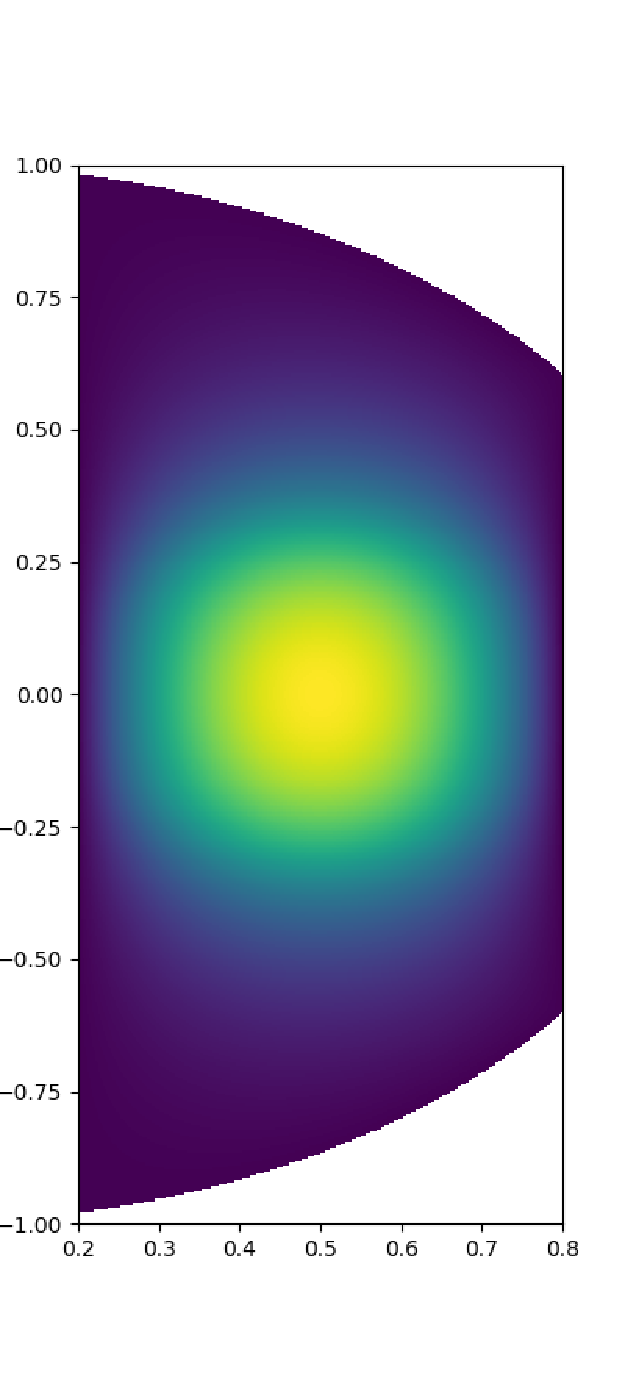
\includegraphics[scale=0.7]{solution-poisson-diskslice-alpha=0p2-beta=0p8}
%	\centering
%	%\label{fig:solution-poisson}
%	\end{subfigure}
%	\centering
%	\begin{subfigure}{0.3\textwidth}
%	\centering
%	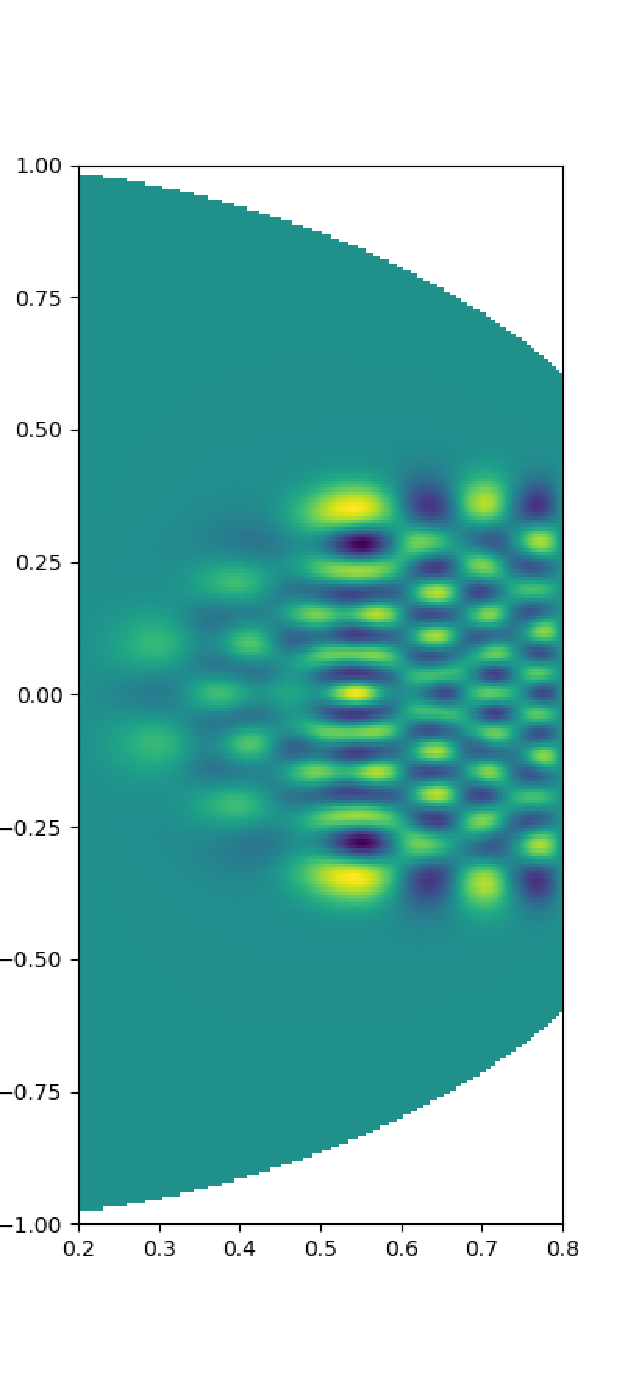
\includegraphics[scale=0.7]{solution-helmholtz-diskslice-alpha=0p2-beta=0p8-k=100-n=300}
%	%\label{fig:solution-helmholtz}
%	\end{subfigure}
%	\begin{subfigure}{0.3\textwidth}
%	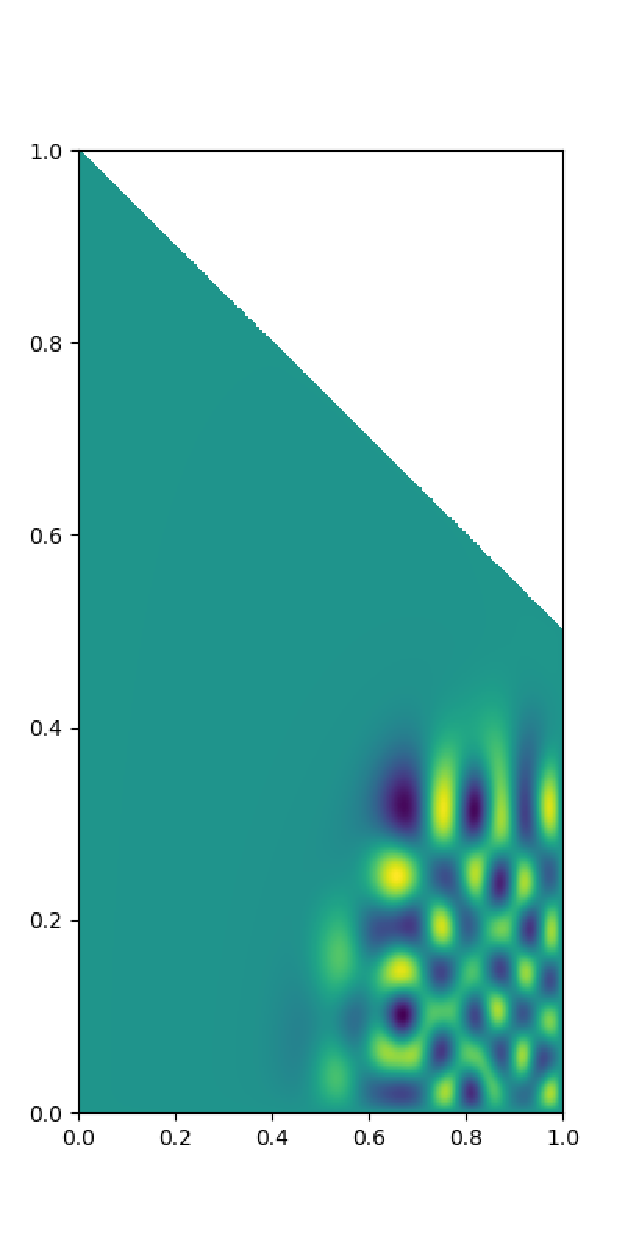
\includegraphics[scale=0.8]{solution-trapezium-helmholtz-k=100-n=1500}
%	%\label{fig:solution-poisson}
%	\centering
%	\end{subfigure}
%	\caption{Left: The computed solution to $\Delta u = f$ with zero boundary conditions with $f(x,y) = 1 + \text{erf}(5(1 - 10((x - 0.5)^2 + y^2)))$. Centre: The computed solution to $\Delta u + k^2 \: v \: u = f$ with zero boundary conditions with $f(x,y) = x(1-x^2-y^2)e^x$, $v(x,y) = 1 - (3(x-1)^2 + 5y^2)$ and $k = 100$. Right: The computed solution to $\Delta u + k^2 \: v \: u = f$ with zero boundary conditions with $f(x,y) = (1-x) \: x \: y \: (1- \half x - y) \: e^x$, $v(x,y) = 1 - (3(x-1)^2 + 5y^2)$ and $k = 100$ in the trapezium. Code utilises ApproxFun \cite{ApproxFun}}
%	\centering
%	\label{fig:solutions}
%\end{wrapfigure}
%
%\begin{wrapfigure}{R}{0.7\textwidth}
%	\centering
%	\begin{subfigure}{0.2\textwidth}
%	\centering
%	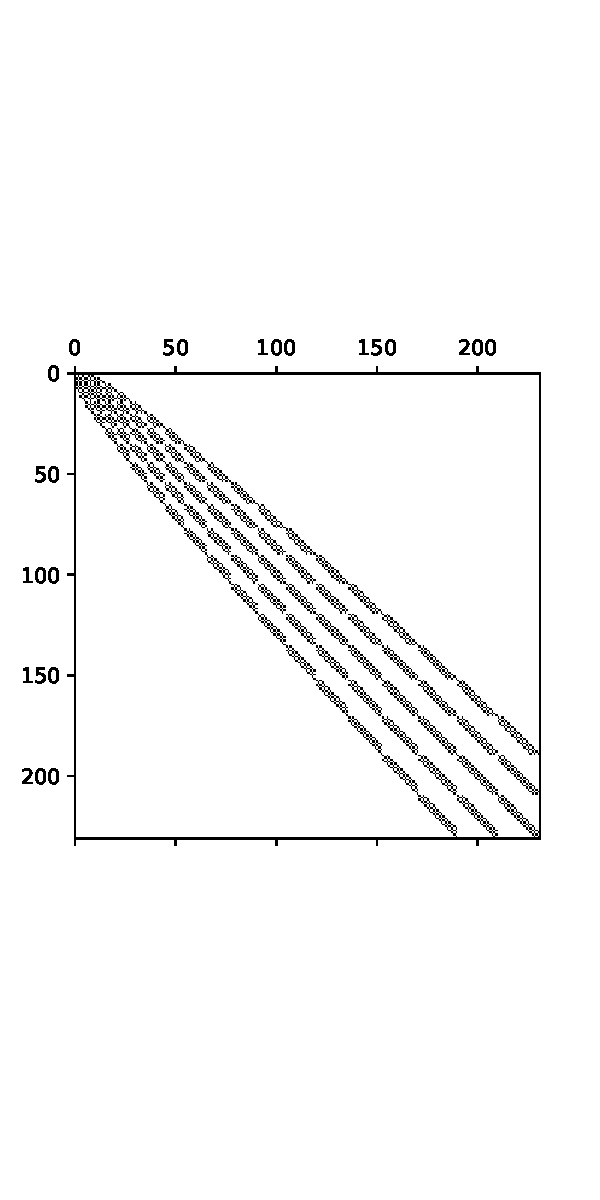
\includegraphics[scale=0.6]{sparsityoflaplacian-w11-diskslice-alpha=0p2-beta=0p8}
%        \centering
%	\end{subfigure}
%	\begin{subfigure}{0.2\textwidth}
%	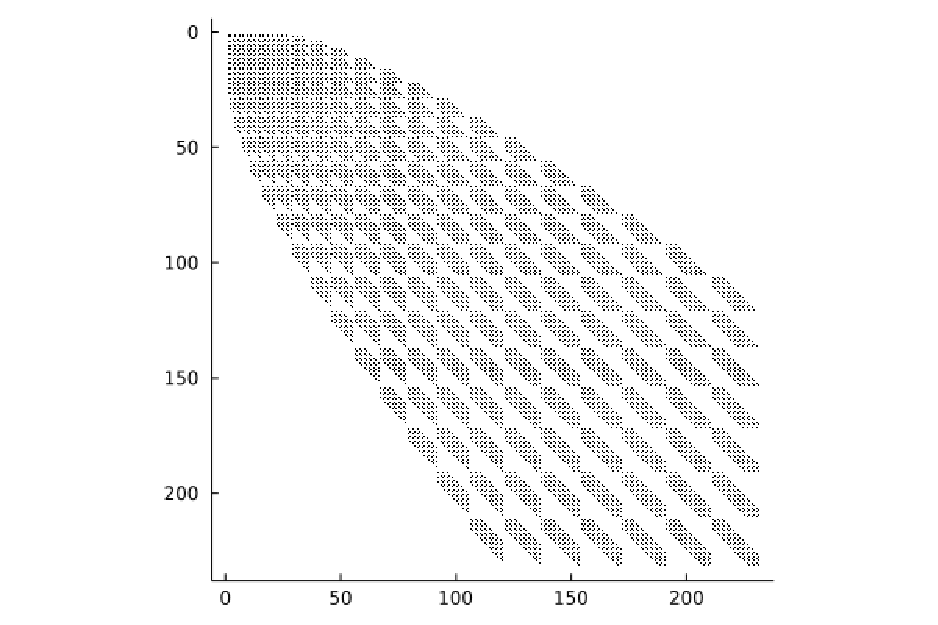
\includegraphics[scale=0.6]{sparsityofhelmholtz-diskslice-alpha=0p2-beta=0p8}
%        \centering
%	\end{subfigure}
%	\begin{subfigure}{0.2\textwidth}
%	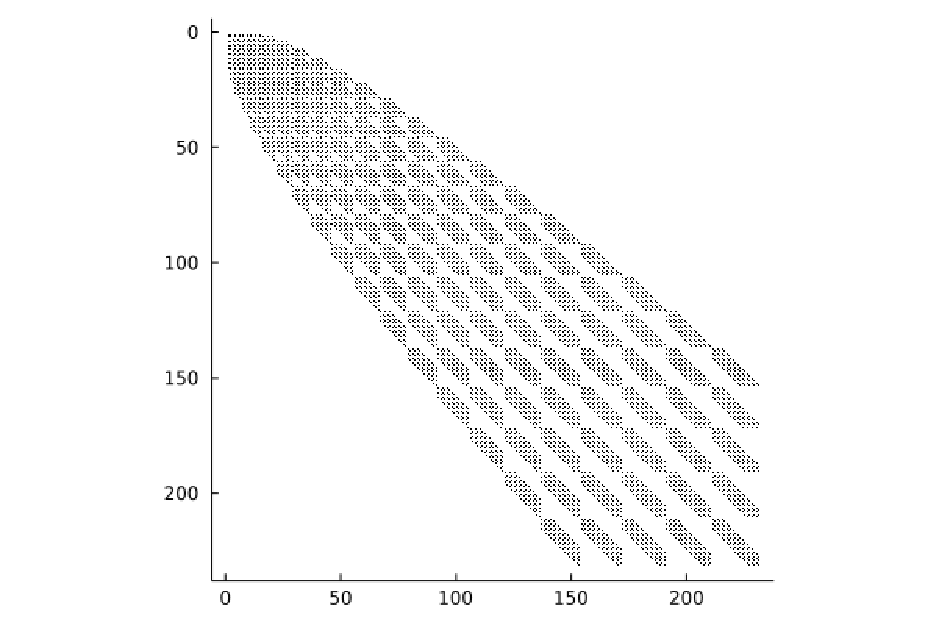
\includegraphics[scale=0.6]{sparsityofbiharmonic-diskslice-alpha=0p2-beta=0p8}
%        \centering
%	\end{subfigure}
%    	\caption{"Spy" plots of (differential) operator matrices, showing their sparsity. Left: the Laplace operator. Centre: the weighted variable coefficient Helmholtz operator $\Delta + k^2 \: v$ for $v(x,y) = 1 - (3(x-1)^2 + 5y^2)$ and $k = 200$. Right: the biharmonic operator.}
%        \label{fig:sparsity}
%        \centering
%\end{wrapfigure}
%
%\begin{wrapfigure}{R}{0.6\textwidth}
%	\centering
%	\begin{subfigure}{0.5\textwidth}
%	\centering
%	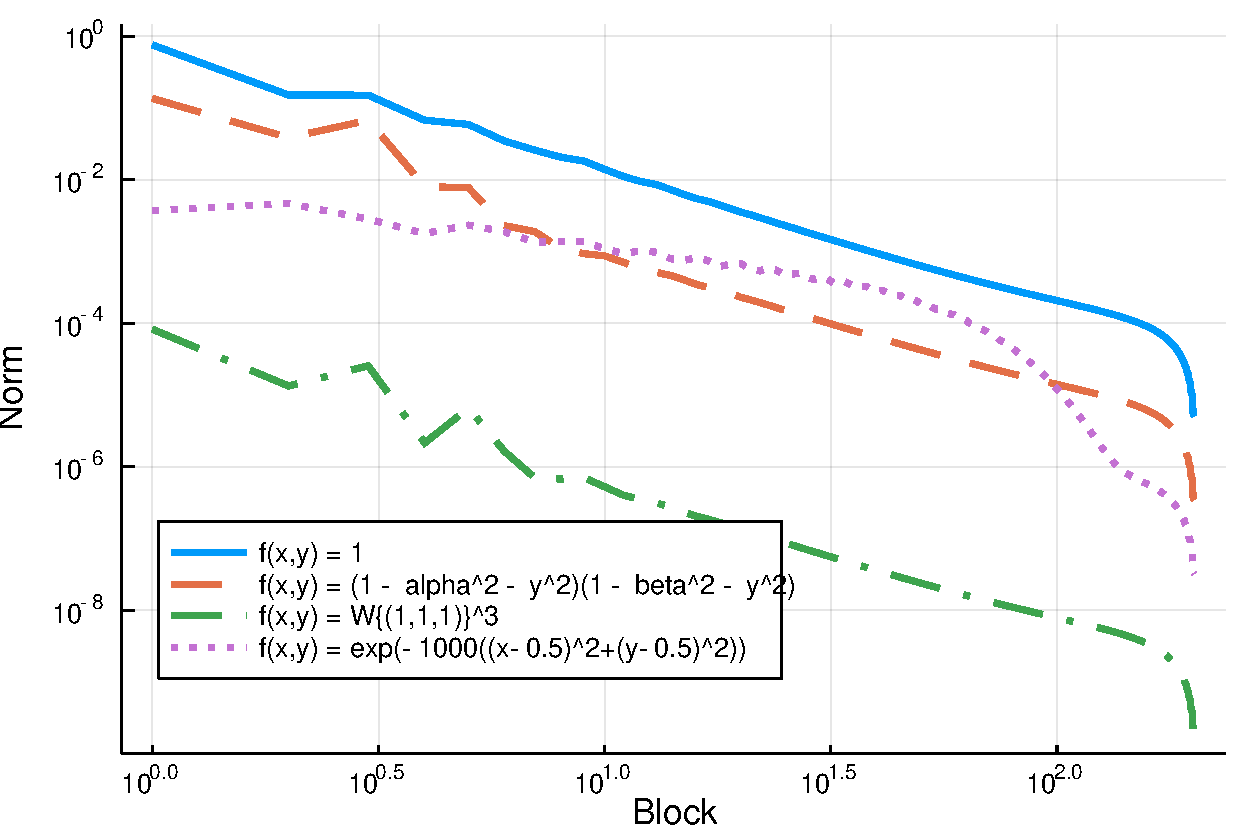
\includegraphics[scale=0.7]{solutionblocknorms-poisson-diskslice-alpha=0p2-beta=0p8-N=200}
%        	%\label{fig:solutionblocknorms-poisson}
%	\end{subfigure}
%	\caption{The norms of each block of the computed solution of the Poisson equation with the given right hand side functions. This demonstrates algebraic convergence with the rate dictated by the decay at the corners, with spectral convergence observed when the right-hand side vanishes to all orders. Code utilises ApproxFun \cite{ApproxFun}}
%	\centering
%	\label{fig:solutionblocknorms}
%\end{wrapfigure}
%
%    }


\end{document}
